














\formatChapter{Pink Tag Boulders}


	\setbox0=\hbox{\begin{overpic}[width=0.8\linewidth]{./maps/area/out/Pink Tag_c.png}
	\end{overpic}}
	\needspace{\ht0}
	\begin{center}
	\begin{overpic}[width=0.9\linewidth]{./maps/area/out/Pink Tag_c.png}\label{sm:Pink Tag area map}
	\end{overpic}
	\end{center}


\raggedcolumns
\begin{multicols}{2}
\qrcode{./maps/qr//Pink Tag Boulders_qr.png}{http://maps.google.com/maps?q=44.43998124232581,-122.57539325959186}{Navigate to this area}
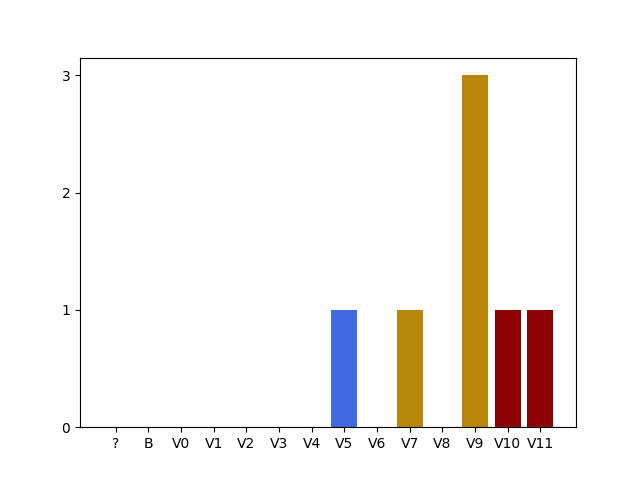
\includegraphics[width=\linewidth]{./maps/plots//Pink Tag Boulders.png}
\end{multicols}
\begin{multicols}{2}



Just across the road from the main area lay a few boulders on the banks of the River. Beware at very high cfs most of the area will be underwater. Since the River is dam controlled the water level can shift rapidy. Consult the USGS flow charts for below green peter damn to know when the river will be low. See driving directions for the Garden Main area.\\

\textbf{NOTE: This area is mostly incomplete. Look forward to more information in future revisions of this book or contribute your own knowledge on github.}\\






	\setbox0=\hbox{\begin{overpic}[width=0.8\linewidth]{./maps/topos/pissings_c.png}
	\end{overpic}}
	\needspace{\ht0}
	\begin{center}
	\begin{overpic}[width=0.9\linewidth]{./maps/topos/pissings_c.png}\label{tp:Territorial Pissings}
	\end{overpic}
	\end{center}


\needspace{1.5cm}
\subsection*{Pissing Boulder}\label{bf:Pissing Boulder}
This blunt overhanging corner is the first boulder that you walk by when entering Pink Tag.\\
	


\needspace{1.5cm}
\label{rt:Territorial Pissings}
\colorbox{RoyalBlue!20}{
\parbox{0.95\linewidth}{
\hspace{-1ex}\textbf{$\Box$
1 Territorial Pissings V5*  
}}}
\begin{adjustwidth}{1.3em}{}			
PLACEHOLDER
\end{adjustwidth}




	\setbox0=\hbox{\begin{overpic}[width=0.8\linewidth]{./maps/topos/jonah_c.png}
	\end{overpic}}
	\needspace{\ht0}
	\begin{center}
	\begin{overpic}[width=0.9\linewidth]{./maps/topos/jonah_c.png}\label{tp:Jonah's Dab Rig}
	\end{overpic}
	\end{center}


\needspace{1.5cm}
\subsection*{Jonah's Dab Rig}\label{bf:Jonah's Dab Rig}
	


\needspace{1.5cm}
\label{rt:Jonah's Dab Rig}
\colorbox{Goldenrod!20}{
\parbox{0.95\linewidth}{
\hspace{-1ex}\textbf{$\Box$
2 Jonah's Dab Rig V9 \ding{72}\ding{72} 
}}}
\begin{adjustwidth}{1.3em}{}			
PLACEHOLDER
\end{adjustwidth}


\begin{adjustwidth}{0.5cm}{}				
\needspace{3cm}
\textbf{Variations:} \newline

\needspace{1.5cm}
\label{vr:Workshop 68}
\colorbox{red!20}{
\parbox{0.95\linewidth}{
\hspace{-1ex}\textbf{$\Box$
2a Workshop 68 V11*  
}}}
\begin{adjustwidth}{1.3em}{}			
PLACEHOLDER
\end{adjustwidth}



\end{adjustwidth}


	\setbox0=\hbox{\begin{overpic}[width=0.8\linewidth]{./maps/topos/fratHouse_c.png}
	\end{overpic}}
	\needspace{\ht0}
	\begin{center}
	\begin{overpic}[width=0.9\linewidth]{./maps/topos/fratHouse_c.png}\label{tp:Frat House}
	\end{overpic}
	\end{center}


\needspace{1.5cm}
\subsection*{Frat House}\label{bf:Frat House}
	


\needspace{1.5cm}
\label{rt:Frat House}
\colorbox{green!20}{
\parbox{0.95\linewidth}{
\hspace{-1ex}\textbf{$\Box$
3 Frat House V2*  
}}}
\begin{adjustwidth}{1.3em}{}			
PLACEHOLDER
\end{adjustwidth}




\needspace{1.5cm}
\label{rt:Frat Mouse}
\colorbox{green!20}{
\parbox{0.95\linewidth}{
\hspace{-1ex}\textbf{$\Box$
4 Frat Mouse V1*  
}}}
\begin{adjustwidth}{1.3em}{}			
PLACEHOLDER
\end{adjustwidth}



	\end{multicols}
	\setbox0=\hbox{\begin{overpic}[width=0.8\linewidth]{./maps/topos/farley_c.png}
	\end{overpic}}
	\needspace{\ht0}
	\begin{center}
	\begin{overpic}[width=0.9\linewidth]{./maps/topos/farley_c.png}\label{tp:Farley}
	\end{overpic}
	\end{center}
	\raggedcolumns
	\begin{multicols}{2}


\needspace{1.5cm}
\label{rt:Belushi}
\colorbox{RoyalBlue!20}{
\parbox{0.95\linewidth}{
\hspace{-1ex}\textbf{$\Box$
5 Belushi V5*  
}}}
\begin{adjustwidth}{1.3em}{}			
PLACEHOLDER
\end{adjustwidth}




\needspace{1.5cm}
\label{rt:Lippity Split}
\colorbox{RoyalBlue!20}{
\parbox{0.95\linewidth}{
\hspace{-1ex}\textbf{$\Box$
6 Lippity Split V5*  
}}}
\begin{adjustwidth}{1.3em}{}			
PLACEHOLDER
\end{adjustwidth}




\needspace{1.5cm}
\label{rt:Le Lemét}
\colorbox{Goldenrod!20}{
\parbox{0.95\linewidth}{
\hspace{-1ex}\textbf{$\Box$
7 Le Lemét V9*  
}}}
\begin{adjustwidth}{1.3em}{}			
PLACEHOLDER
\end{adjustwidth}




\needspace{1.5cm}
\label{rt:Farley Prep}
\colorbox{Goldenrod!20}{
\parbox{0.95\linewidth}{
\hspace{-1ex}\textbf{$\Box$
8 Farley Prep V9*  
}}}
\begin{adjustwidth}{1.3em}{}			
PLACEHOLDER
\end{adjustwidth}


\begin{adjustwidth}{0.5cm}{}				
\needspace{3cm}
\textbf{Variations:} \newline

\needspace{1.5cm}
\label{vr:Knowledge is Good}
\colorbox{Goldenrod!20}{
\parbox{0.95\linewidth}{
\hspace{-1ex}\textbf{$\Box$
8a Knowledge is Good V7*  
}}}
\begin{adjustwidth}{1.3em}{}			
PLACEHOLDER
  (No Topo)
\end{adjustwidth}



\end{adjustwidth}




\end{multicols}
\clearpage